\section{Connections on Bundles}
Let's just look at a local neighborhood $U$ around point $p$ where we have a coordinate system $(x_0, x_1, ..., x_n)$ on our vector bundle of interest.  Given this coordinate system, we can create derivatives
\begin{equation}
  \text{d}f = \d{f}{x_0} \text{d}x_0 + \d{f}{x_1} \text{d}x_1 + ... + \d{f}{x_n} \text{d}x_n
\end{equation}
given some function $f$ through the point of interest $p$ in the neighborhood $U$. The vector $(\d{}{x_0}, \d{}{x_1},...,\d{}{x_n}) $ defines the \textbf{Tangent space}, and the covector $(\text{d} x_0, \text{d}x_1, ..., \text{d} x_n)$ defines the \textbf{Cotangent space} at point $p$.

The next step takes a bit of adjustment to understand.  We have to make a \textit{choice}.  Just like how we imposed extra structure on sets to create topologies, or on topologies to make bundles, we now have to impose extra structure on our bundle that does not intrinsically exist.  Without making this \textit{choice}, we actually do not have anyway to connect to fibers adjacent to each other on the same bundle.

  \begin{wrapfigure}{L}{.4\textwidth}\begin{center}
    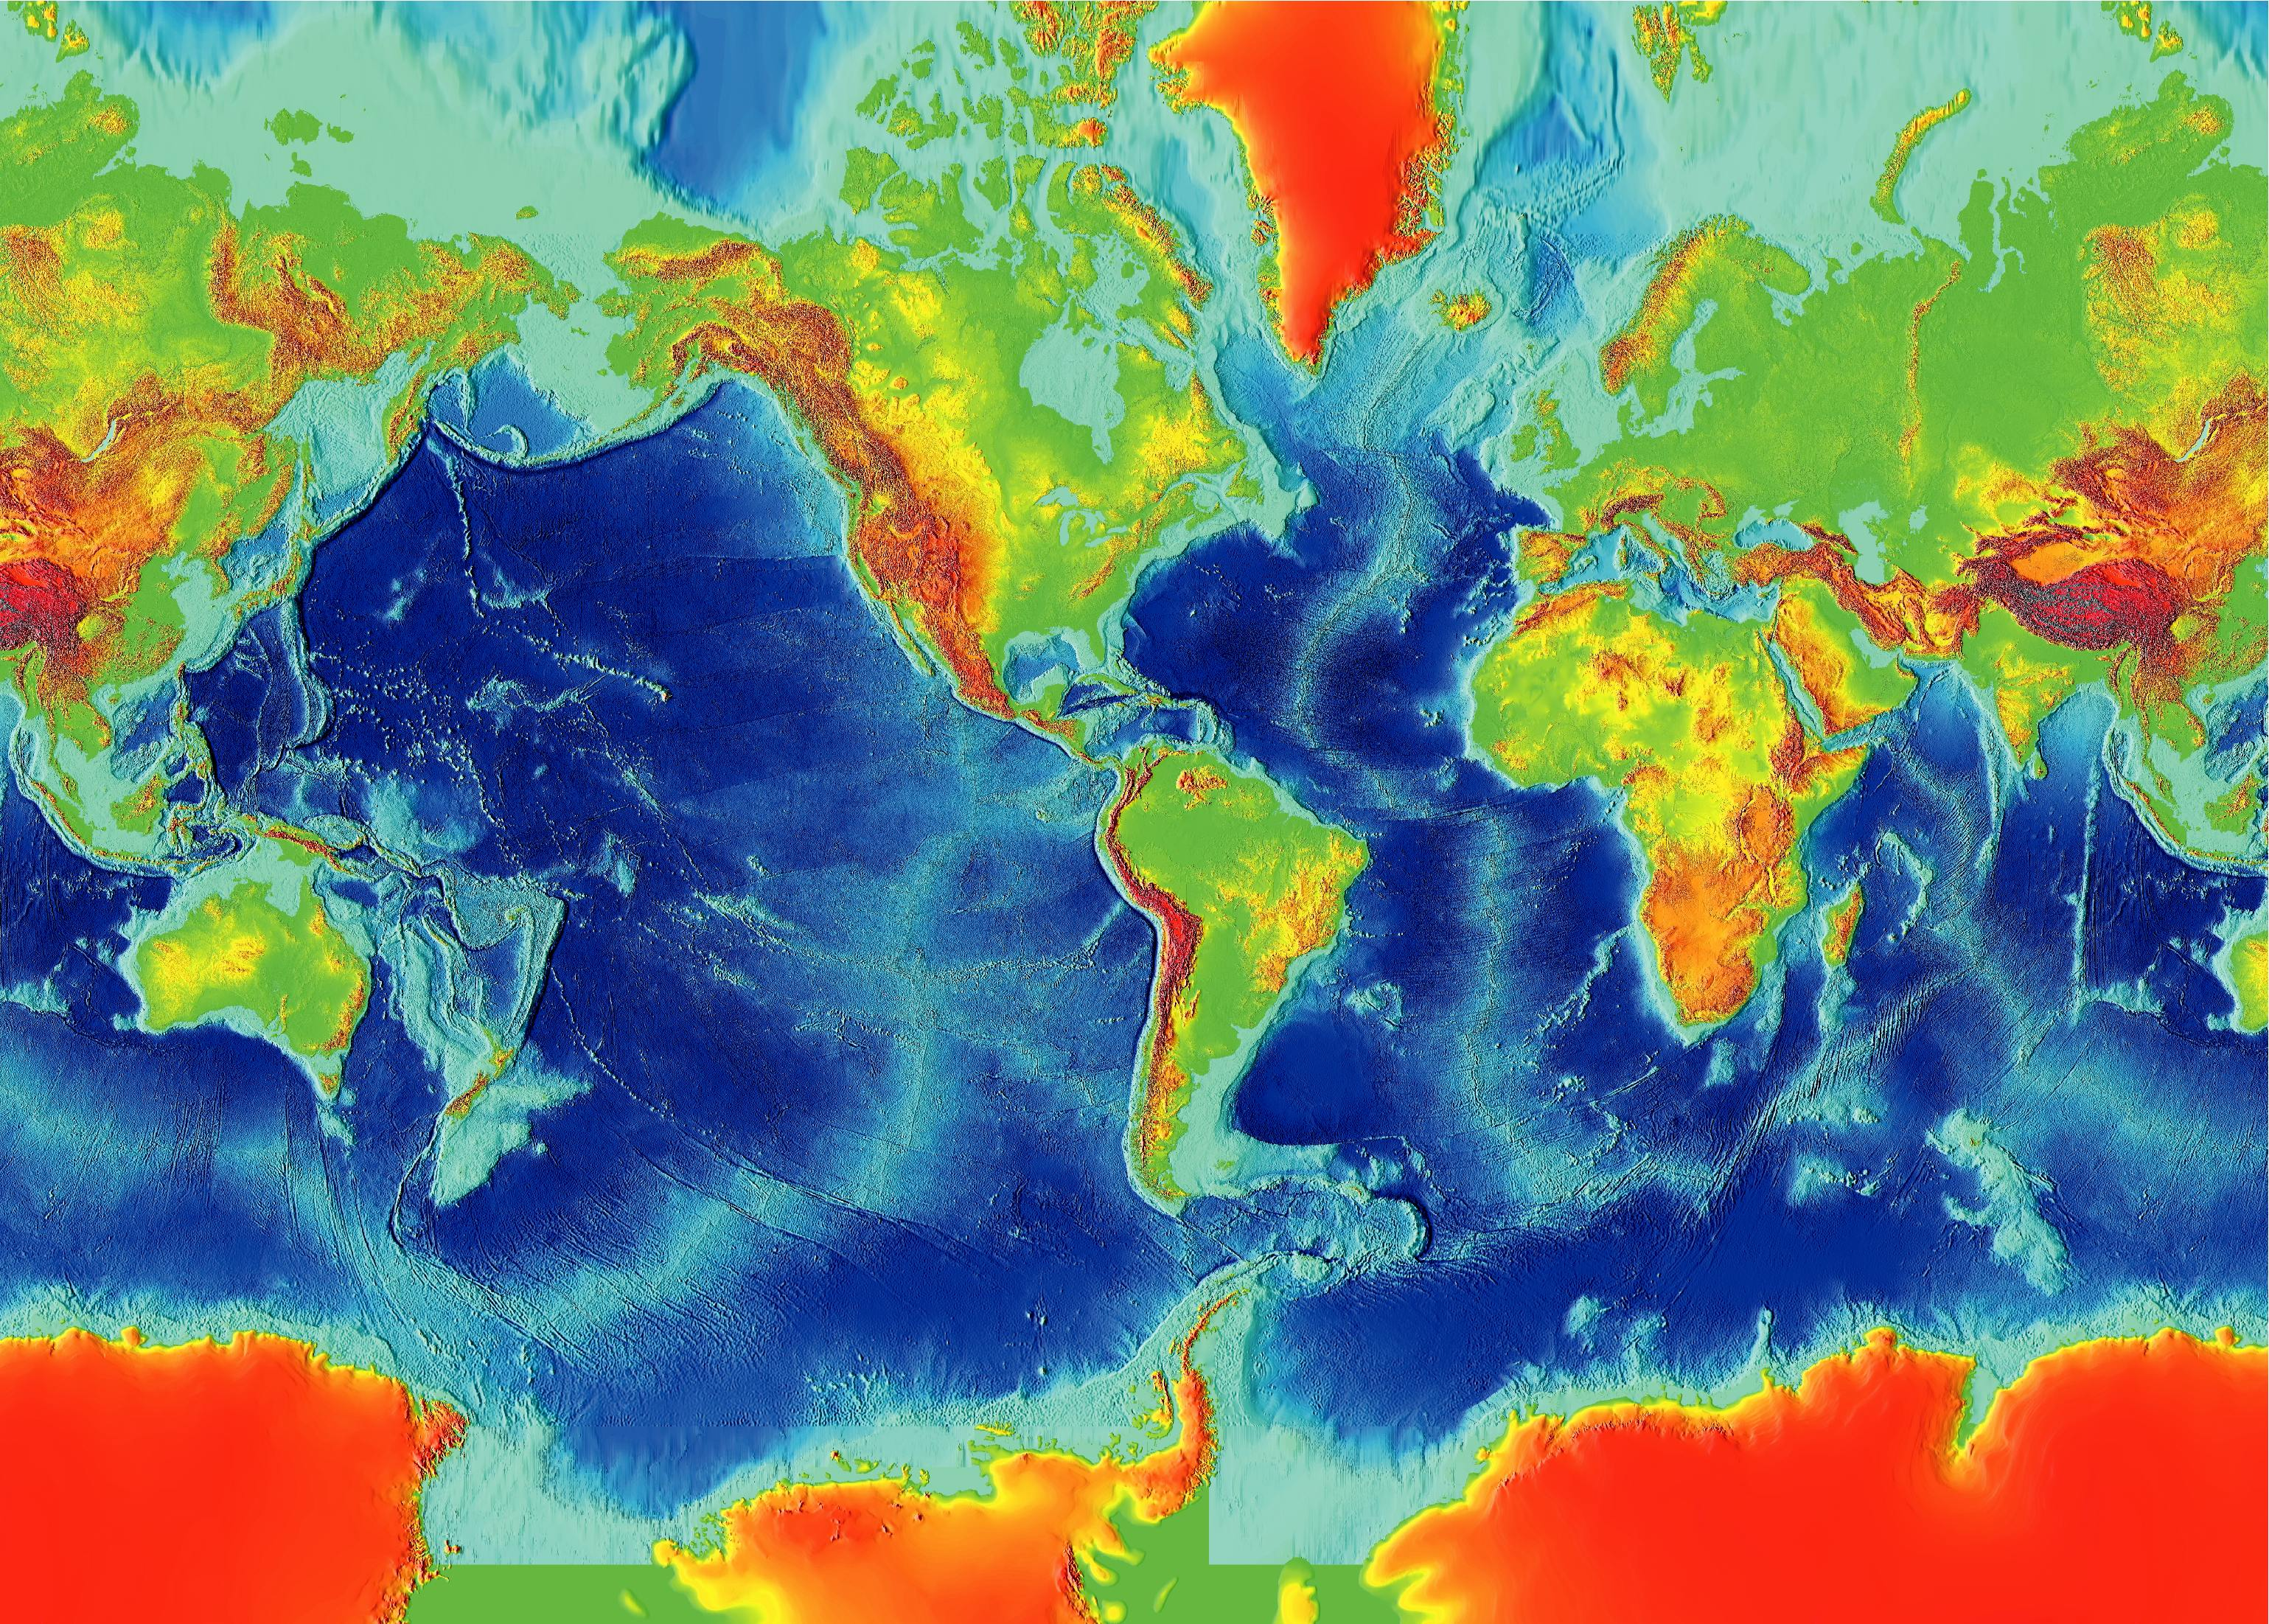
\includegraphics[width=.35\textwidth]{pics/earth_surface.jpg}\end{center}
    \caption{ \protect\footnotemark }
  \end{wrapfigure}
\footnotetext{File:Earth surface NGDC 2000.jpg|Earth surface NGDC 2000}

  Normally we describe the Earth as just a perfect sphere, $S^2$, but it's not.  So let us instead describe it as a fiber bundle where each point of the base manifold of $S^2$ has possible heights associated with it pulled from $\mathbb{R}$.  The surface of the Earth will be a section defined on the sphere. We can see those values in the elevation map to the right.

  Only after we define the surface of the Earth can we say what vectors go along the surface of the Earth, what vectors are perpendicular (complimentary to the surface) to the Earth, and how I would get to the top of Fuji-yama.  If I assumed the Earth was a perfect sphere, climbing Fuji-yama would land me deep in some pretty toxic substances.  I have to account for how moving horizontally means I acquire some vertical change.

\begin{figure}
  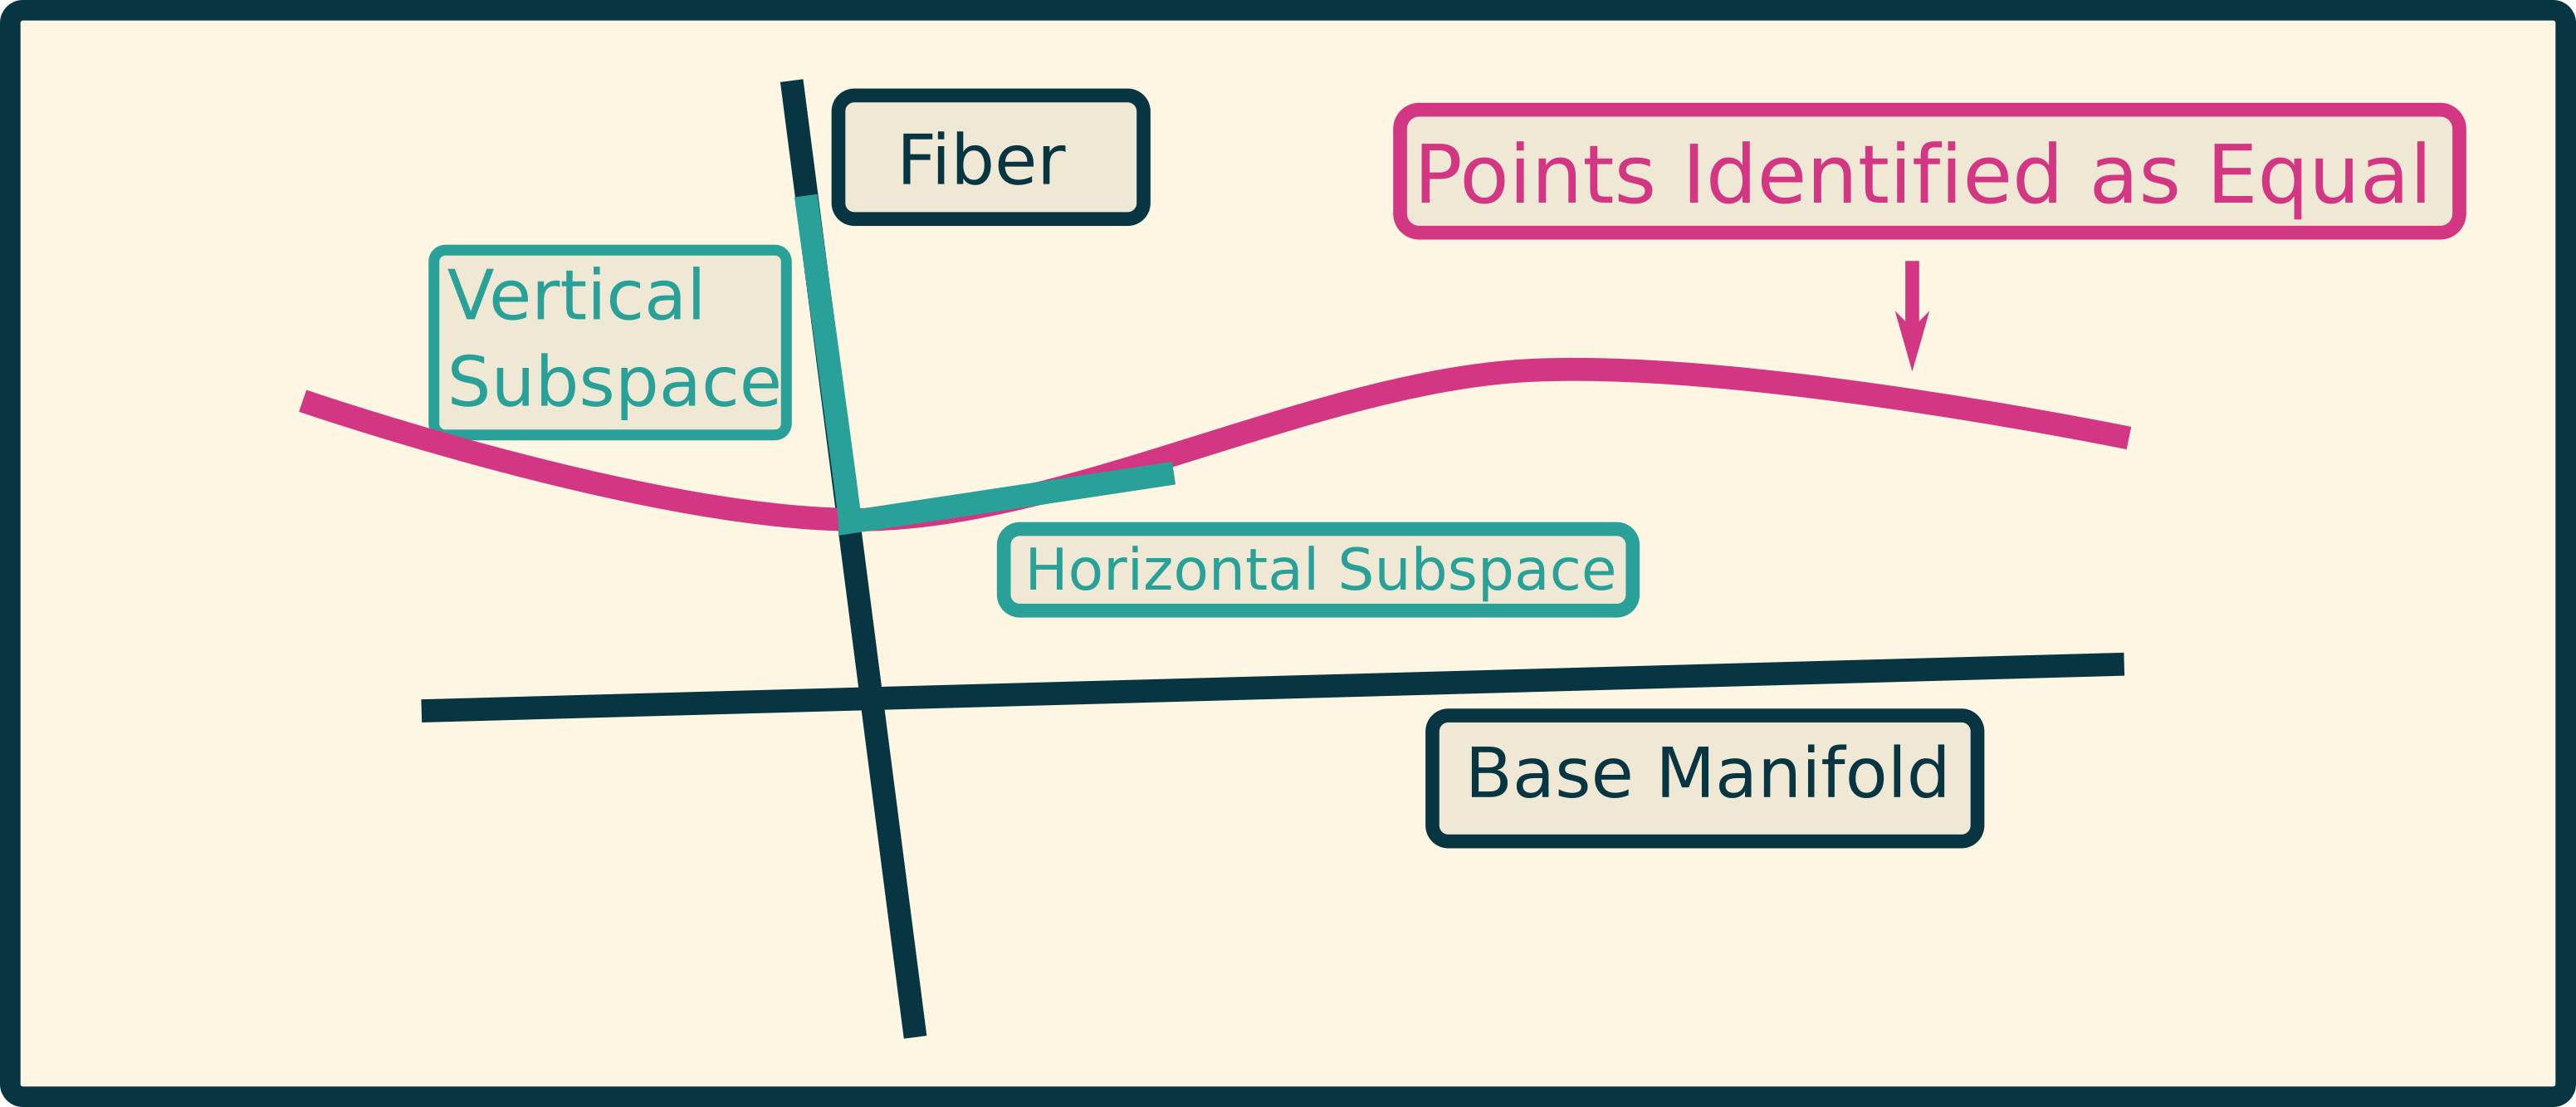
\includegraphics[width=\textwidth]{pics/bundle_tangent.png}
  \caption{Once we identify which points in the topology are identical, we can separate out the tangent space at each point into the horizontal and vertical components.}
  \label{fig:bundle_tangent}
\end{figure}

Identifying 
